\FloatBarrier
\section{Auswertung}
\label{sec:Auswertung}

In der Tabelle \ref{tab:Messwerte} sind die Messwerte von
$R_{Probe}$ und $R_{Mantel}$ zur Messzeit $t$ aufgelistet.
Aus dem Zusammenhang
\begin{align}
  T=\num{0.00134} R_i^2 + \num{2.296} R_i - \num{30.1} \label{eqn:inKelvin}
\end{align}
kann aus den Messwerten der Widerstände
die Temperatur der Probe und
des Mantels errechnet werden, die ebenfalls in der
Tabelle \ref{tab:Messwerte} enthalten sind.
Die Abbildung \ref{fig:T_mess} zeigt den
Verlauf des Aufheizens sowohl von der Probe
als auch des Mantels.



\begin{table}  % Messwerte
  \centering
  \caption{Messwerte der Widerstände $R_i$ und die daraus resultierenden Temperaturen $T_i$ für Mantel und Probe und die Betragsmäßige Temperaturdifferenz zwischen Mantel und Probe.}
  \label{tab:Messwerte}
  \begin{tabular}{c c c c c c}
  \toprule
  $t/\si{\second}$ & $R_{Probe}/\si{\ohm}$ & $T_{Probe}/\si{\kelvin}$ & $R_{Mantel}/\si{\ohm}$ & $T_{Mantel}/\si{\kelvin}$ & $|T_{Mantel}-T_{Probe}|/\si{\kelvin}$\\
  \midrule
  0	&	23.8	&	85.5	&	22.4	&	82.2	&	3.3   \\
  150	&	26.0	&	90.7	&	23.9	&	85.8	&	5.0   \\
  300	&	28.0	&	95.5	&	27.2	&	93.6	&	1.9   \\
  450	&	29.5	&	99.0	&	30.1	&	100.4	&	1.4   \\
  600	&	31.3	&	103.3	&	34.0	&	109.7	&	6.4   \\
  750	&	33.2	&	107.8	&	36.9	&	116.7	&	8.8   \\
  900	&	35.1	&	112.4	&	38.7	&	121.0	&	8.6   \\
  1050	&	37.0	&	116.9	&	40.1	&	124.3	&	7.4   \\
  1200	&	38.7	&	121.0	&	41.1	&	126.7	&	5.8   \\
  1350	&	40.3	&	124.8	&	42.2	&	129.4	&	4.6   \\
  1500	&	43.4	&	132.3	&	44.3	&	134.5	&	2.2   \\
  1800	&	46.2	&	139.0	&	45.4	&	137.1	&	1.9   \\
  2100	&	48.9	&	145.6	&	49.5	&	147.0	&	1.5   \\
  2400	&	51.8	&	152.6	&	53.0	&	155.6	&	2.9   \\
  2700	&	54.5	&	159.2	&	53.7	&	157.3	&	2.0   \\
  3000	&	57.0	&	165.3	&	54.7	&	159.7	&	5.6   \\
  3300	&	59.4	&	171.2	&	58.3	&	168.5	&	2.7   \\
  3600	&	62.0	&	177.6	&	62.5	&	178.8	&	1.2   \\
  3900	&	64.5	&	183.8	&	64.6	&	184.0	&	0.2   \\
  4200	&	67.1	&	190.2	&	67.9	&	192.2	&	2.0   \\
  4500	&	69.8	&	196.9	&	69.4	&	195.9	&	1.0   \\
  4800	&	72.1	&	202.6	&	69.9	&	197.1	&	5.5   \\
  5100	&	74.4	&	208.3	&	73.7	&	206.6	&	1.7   \\
  5400	&	76.9	&	214.6	&	79.0	&	219.8	&	5.3   \\
  5700	&	81.9	&	227.1	&	81.9	&	227.1	&	0.0   \\
  6000	&	84.2	&	232.9	&	84.1	&	232.6	&	0.3   \\
  6300	&	86.6	&	238.9	&	87.6	&	241.5	&	2.5   \\
  6600	&	89.2	&	245.5	&	89.1	&	245.3	&	0.3   \\
  6900	&	91.2	&	250.6	&	89.5	&	246.3	&	4.3   \\
  7200	&	93.3	&	255.9	&	92.6	&	254.1	&	1.8   \\
  7500	&	95.6	&	261.8	&	96.5	&	264.1	&	2.3   \\
  7800	&	98.6	&	269.4	&	98.5	&	269.2	&	0.3   \\
  8100	&	100.4	&	274.1	&	100.2	&	273.5	&	0.5   \\
  8400	&	102.6	&	279.7	&	102.6	&	279.7	&	0.0   \\
  8700	&	105.0	&	285.9	&	105.5	&	287.2	&	1.3   \\
  9000	&	107.2	&	291.5	&	106.8	&	290.5	&	1.0   \\
  9300	&	109.5	&	297.5	&	109.1	&	296.5	&	1.0   \\

  \bottomrule
\end{tabular}
\end{table}

\begin{figure}
  \centering
  \includegraphics{build/temperatur_verlauf.pdf}
  \caption{Temperatur von Mantel und Probe in Abhängigkeit der Zeit $t$.}
  \label{fig:T_mess}
\end{figure}


Als Heizstrom und Heizspannung der Probe
werden
\begin{align}
  I = \SI{152(2)}{\milli\ampere}
  U = \SI{16.0(5)}{\volt}
\end{align}
verwendet. Die Größe
der Fehler auf Heizstrom und Heizspannung
sind nicht der Messgeräten geschuldet,
sondern resultieren daher, dass nicht
zu jedem gemessenen Widerstandswert
zusätzlich Heizstrom und Heizspannung
aufgenommen wurden, jedoch später
eine leichte Abhängigkeit
der Größen festgestellt wurde.
Über die Heizleistung $P=UI$
und die Zeitdifferenz $\delta t$
kann die Energie, die der Probe zugeführt wird
und diese um die Temperaturdifferenz
$\delta T$ aufwärmt, bestimmt werden.
Für die Molwärme bei konstantem
Druck $C_p$ ergibt sich somit
\begin{align}
  C_p =\frac{\text{d} Q}{n \text{d} T }  = \frac{UI \cdot \Delta t \rho V_m }{m \Delta T}. \label{eqn:C_p}
\end{align}
Aus dem Zusammenhang
\begin{align}
C_V = C_P- 9\alpha^2 \kappa V_0 T \label{eqn:C_V}.
\end{align}
folgt die Molwärme bei konstantem Volumen.
Der lineare Ausdehnungskoeffizient $\alpha$ besitzt dabei
eine Temperatur Abhängigkeit die in der Tabelle \ref{fig:alpha}
aufgelistet ist. Um für Temperaturzwischenwerte von $\alpha$
zu berechnen, wird an die Werte aus der Tabelle \ref{fig:alpha}
eine Polynom 4. Grades
\begin{align}
f(T) = a T^4 + b  T^3 + c  T^2 + d T + e \label{eqn:poly4}
\end{align}
gefittet.
Es ergeben sich die folgenden Fitparameter:
\begin{align}
 a&=\SI{-8.2(7)e-15}{}
  & b&=\SI{7.4(5)e-12}{}   & c &=\SI{-2.5(1)e-9}{}  \\
 d&=\SI{4.1(2)e-7}{}    & e&=\SI{-1.1(1)e-5}{}
\end{align}
\begin{table}
  \centering
  \caption{Linearer Ausdehnungskoeffizient von Kupfer in Abhängigkeit von der Temperatur.}
  \label{fig:alpha}
  \centering
  \begin{tabular}{c}
  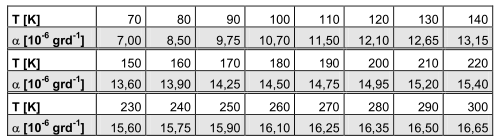
\includegraphics[width=0.7\textwidth]{alpha.PNG}
\end{tabular}
\end{table}

Die Tabelle \ref{tab:C_P_C_V} enthält die berechneten Werte von $C_p$ nach Gleichung \eqref{eqn:C_p} und $C_V$ nach Gleichung \eqref{eqn:C_V}.
Wobei für die Temperatur bei der $C_V$ Berechnung ein $T_{mittel}$ verwendet wird, was sich aus den Temperaturen $T_{probe}$ aus Tabelle \ref{tab:Messwerte}
mit der Gleichung
\begin{align}
  T_{mittel} = \left(T_1 + \frac{T_2-T_1}{2}\right)  \pm \frac{T_2-T_1}{2}
\end{align}
ergibt.

\begin{table}  %   Messwerte_C_P_C_V
  \centering
  \caption{Molwärem $C_P$ bei konstantem
   Druck und alle benötigten Werte, um nach Gleichung
  \eqref{eqn:C_V} die Molwärme $C_V$ zu bestimmen und der berechnete Wert von $C_V$ selbst .}
  \label{tab:C_P_C_V}
  \begin{tabular}{c c c c c c}
    \toprule
    $\Delta t/\si{\second}$ & $\Delta T/ \si{\kelvin}$ & $C_p/ \si{\joule\per\mol\per\kelvin}$ & $T_{mittel}/ \si{\kelvin}$ & $\alpha/\si{\per\kelvin}$ & $C_V/ \si{\joule\per\mol\per\kelvin}$\\
    \midrule
    150	&	5.2	&	13.02	\pm	0.44	&	88.1	\pm	2.6	&	9.44	\pm0.29	&	12.95	\pm 0.44   \\
    150	&	4.7	&	14.29	\pm	0.48	&	93.1	\pm	2.4	&	9.97	\pm0.24	&	14.20	\pm 0.48   \\
    150	&	3.6	&	19.01	\pm	0.64	&	97.2	\pm	1.8	&	10.38	\pm	0.17	&	18.92	\pm	0.64   \\
    150	&	4.3	&	15.81	\pm	0.54	&	101.2	\pm	2.1	&	10.74	\pm	0.19	&	15.71	\pm	0.54   \\
    150	&	4.5	&	14.95	\pm	0.51	&	105.6	\pm	2.3	&	11.11	\pm	0.18	&	14.83	\pm	0.51   \\
    150	&	4.5	&	14.92	\pm	0.51	&	110.1	\pm	2.3	&	11.47	\pm	0.17	&	14.79	\pm	0.51   \\
    150	&	4.5	&	14.89	\pm	0.50	&	114.6	\pm	2.3	&	11.79	\pm	0.16	&	14.74	\pm	0.50   \\
    150	&	4.1	&	16.60	\pm	0.56	&	118.9	\pm	2.0	&	12.08	\pm	0.13	&	16.45	\pm	0.56   \\
    150	&	3.8	&	17.61	\pm	0.60	&	122.9	\pm	1.9	&	12.33	\pm	0.11	&	17.44	\pm	0.60   \\
    150	&	7.5	&	9.06	\pm	0.31	&	128.6	\pm	3.7	&	12.65	\pm	0.20	&	8.88	\pm 0.31   \\
    300	&	6.8	&	20.01	\pm	0.68	&	135.7	\pm	3.4	&	13.00	\pm	0.16	&	19.80	\pm	0.68   \\
    300	&	6.5	&	20.69	\pm	0.70	&	142.3	\pm	3.3	&	13.30	\pm	0.14	&	20.46	\pm	0.70   \\
    300	&	7.0	&	19.20	\pm	0.65	&	149.1	\pm	3.5	&	13.57	\pm	0.13	&	18.95	\pm	0.65   \\
    300	&	6.6	&	20.56	\pm	0.70	&	155.9	\pm	3.3	&	13.81	\pm	0.11	&	20.29	\pm	0.70   \\
    300	&	6.1	&	22.14	\pm	0.75	&	162.3	\pm	3.1	&	14.02	\pm	0.09	&	21.86	\pm	0.75   \\
    300	&	5.9	&	23.00	\pm	0.78	&	168.3	\pm	2.9	&	14.19	\pm	0.08	&	22.70	\pm	0.78   \\
    300	&	6.4	&	21.18	\pm	0.72	&	174.4	\pm	3.2	&	14.36	\pm	0.08	&	20.85	\pm	0.72   \\
    300	&	6.2	&	21.96	\pm	0.74	&	180.7	\pm	3.1	&	14.51	\pm	0.08	&	21.62	\pm	0.74   \\
    300	&	6.4	&	21.06	\pm	0.71	&	187.0	\pm	3.2	&	14.66	\pm	0.07	&	20.70	\pm	0.71   \\
    300	&	6.7	&	20.22	\pm	0.69	&	193.5	\pm	3.3	&	14.81	\pm	0.07	&	19.84	\pm	0.69   \\
    300	&	5.7	&	23.67	\pm	0.80	&	199.7	\pm	2.9	&	14.94	\pm	0.06	&	23.28	\pm	0.80   \\
    300	&	5.7	&	23.62	\pm	0.80	&	205.4	\pm	2.9	&	15.06	\pm	0.06	&	23.20	\pm	0.80   \\
    300	&	6.2	&	21.67	\pm	0.73	&	211.4	\pm	3.1	&	15.19	\pm	0.06	&	21.23	\pm	0.73   \\
    300	&	12.5&	10.79 \pm	0.37	&	220.8	\pm	6.3	&	15.37	\pm	0.12	&	10.33	\pm	0.37   \\
    300	&	5.8	&	23.37	\pm	0.79	&	230.0	\pm	2.9	&	15.55	\pm	0.06	&	22.87	\pm	0.79   \\
    300	&	6.1	&	22.34	\pm	0.76	&	235.9	\pm	3.0	&	15.67	\pm	0.06	&	21.82	\pm	0.76   \\
    300	&	6.6	&	20.57	\pm	0.70	&	242.2	\pm	3.3	&	15.79	\pm	0.06	&	20.03	\pm	0.70   \\
    300	&	5.1	&	26.68	\pm	0.90	&	248.1	\pm	2.5	&	15.90	\pm	0.05	&	26.11	\pm	0.90   \\
    300	&	5.3	&	25.35	\pm	0.86	&	253.3	\pm	2.7	&	15.99	\pm	0.05	&	24.77	\pm	0.86   \\
    300	&	5.9	&	23.09	\pm	0.78	&	258.9	\pm	2.9	&	16.09	\pm	0.05	&	22.49	\pm	0.78   \\
    300	&	7.7	&	17.66	\pm	0.60	&	265.6	\pm	3.8	&	16.20	\pm	0.06	&	17.03	\pm	0.60   \\
    300	&	4.6	&	29.35	\pm	1.00	&	271.8	\pm	2.3	&	16.30	\pm	0.03	&	28.71	\pm	1.00   \\
    300	&	5.6	&	23.97	\pm	0.81	&	276.9	\pm	2.8	&	16.37	\pm	0.04	&	23.30	\pm	0.81   \\
    300	&	6.2	&	21.92	\pm	0.74	&	282.8	\pm	3.1	&	16.45	\pm	0.04	&	21.23	\pm	0.74   \\
    300	&	5.7	&	23.85	\pm	0.81	&	288.7	\pm	2.8	&	16.51	\pm	0.03	&	23.15	\pm	0.81   \\
    300	&	5.9	&	22.76	\pm	0.77	&	294.5	\pm	3.0	&	16.56	\pm	0.02	&	22.04	\pm	0.77   \\
    \bottomrule
  \end{tabular}
\end{table}

Zu Bestimmung der Debyetemperatur werden nur Messwerte von $C_V(T)$ bis zur einer Temperatur $T_{max}=\SI{170}{\kelvin} $ benutzt werden, dabei werden noch stark abweichende Messwerte vernachlässigt.
Welche Messwerte verwendet werden, ist noch mal genau in Abbildung \ref{fig:cool} zu sehen, sowie
der klassische Wert von $C_V=3R$ und die Werte der Debyefunktion
für den Literaturwert von $\theta_D = \SI{345}{\kelvin}$  \cite{debyetemp}


\begin{figure}
 \centering
 \includegraphics[width=0.7\textwidth]{molwaerme_V_const_und_theo.pdf}
   \caption{ $C_V$ in Abhängigkeit der Temperatur der Messwert und die verschieden Theoriekurven. So wie die Messwerte die zur Bestimmung der Debyetemperatur verwendet werden.}
   \label{fig:cool}
 \end{figure}

 Um aus den verwendeten Werten von $C_V$ aus Abbildung \ref{fig:cool} die Debyetemperatur $\theta_D$ von Kupfer zu bestimmen,
 wird an die Werte der Debyefunktion, die in Tabelle \ref{fig:debye} aufgetragen sind, im Bereich von $\sfrac{C_V}{[C_V]}  \in [14,22]$
 eine Polynom 4. Grades
 \begin{align}
\frac{\theta}{T}  = f(C_V) = a C_V^4 + b  C_V^3 + c  C_V^2 + d C_V + e
 \end{align}
 gefittet.
 Es ergeben sich die folgenden Fitparameter:
 \begin{align}
 a&=\SI{-4.0(3)e-5}{}    & b&=\SI{2.0(2)e-3}{}   & c &=\SI{-0.044(5)}{}  \\
 d&=\SI{0.11(6)}{}    & e&=\SI{6.2(3)}{}
 \end{align}

 Die Abbildung \ref{fig:debye_fit} enthält sowohl
 die Werte der Debyefunktion
 aus der Tabelle \ref{fig:debye} und die Fitfunktion
 $f(C_V)$.

 \begin{table}
  \centering
  \caption{Werte für die Debyefunktion.}
  \label{fig:debye}
\begin{tabular}{c}
  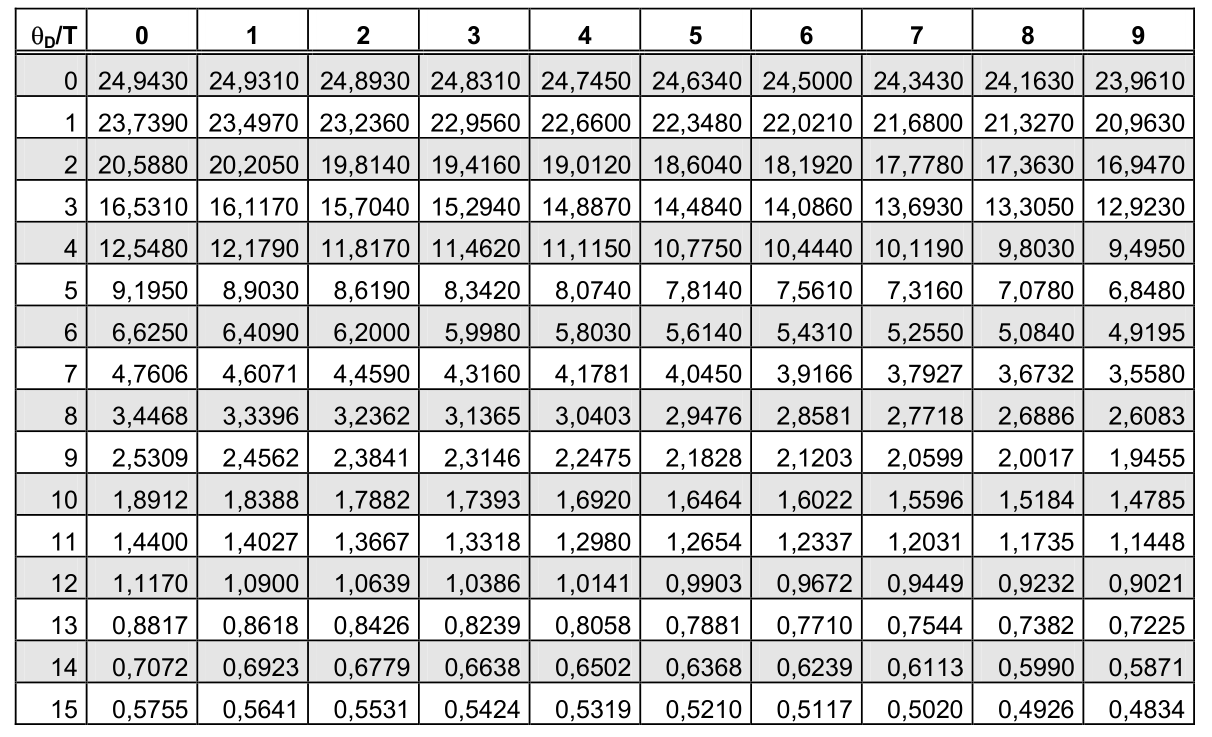
\includegraphics[width=0.9\textwidth]{Debye.PNG}
\end{tabular}
\end{table}

  \begin{figure}
   \centering
   \includegraphics[width=0.7\textwidth]{debyefunktion.pdf}
     \caption{Werte der Debyefunktion und die Fitfunktion
     $f(C_V)$ $\theta_D/T$ in Abhängigkeit von $C_V$.}
     \label{fig:debye_fit}
   \end{figure}



 Die Debyetemperatur $\theta_D$ ergibt sich somit aus
 \begin{align}
   \theta_D = \frac{f(C_V(T))}{T}. \label{eqn:theta_D}
 \end{align}
Die Tabelle \ref{tab:Debyetemperatur} enthält alle
Temperatur bis zur Temperatur $T_{max}$ und die nach Gleichung \eqref{eqn:theta_D}
bestimmte Debyetemperatur $\theta_D$.

\begin{table}
  \centering
  \caption{Berechnete Werte von $C_V$ und entsprechendes Verhältnis
  von $\theta_D/T$ und die gemessene Temperatur $T$ und die über \eqref{eqn:theta_D} berechnete Debyetemperatur $\theta_D$. }
  \label{tab:Debyetemperatur}
  \begin{tabular}{c c c c}
\toprule
$C_V/\si{\joule\per\mol\per\kelvin} $ &  $ \theta_D/T $   &   T/ $\si{\kelvin}$  & $\theta_D/\si{\kelvin}$  \\
\midrule
12.95	 \pm	0.44	&	3.89	\pm	0.11	&	88.1	\pm	2.6	&	342.7	\pm	14.3   \\
14.20	 \pm	0.48	&	3.57	\pm	0.12	&	93.1	\pm	2.4	&	332.4	\pm	14.2   \\
15.71	 \pm	0.54	&	3.20	\pm	0.13	&	101.2	\pm	2.1	&	323.6	\pm	14.9   \\
14.83	 \pm	0.51	&	3.41	\pm	0.13	&	105.6	\pm	2.3	&	360.4	\pm	15.4   \\
14.79	 \pm	0.51	&	3.42	\pm	0.13	&	110.1	\pm	2.3	&	377.0	\pm	15.9   \\
14.74	 \pm	0.50	&	3.44	\pm	0.13	&	114.6	\pm	2.3	&	393.9	\pm	16.4   \\
16.45	 \pm	0.56	&	3.02	\pm	0.14	&	118.9	\pm	2.0	&	359.2	\pm	17.3   \\
17.44	 \pm	0.60	&	2.78	\pm	0.14	&	122.9	\pm	1.9	&	341.8	\pm	18.5   \\
19.80	 \pm	0.68	&	2.20	\pm	0.17	&	135.7	\pm	3.4	&	298.9	\pm	24.6   \\
20.46	 \pm	0.70	&	2.03	\pm	0.18	&	142.3	\pm	3.3	&	289.4	\pm	27.1   \\
18.95	 \pm	0.65	&	2.41	\pm	0.16	&	149.1	\pm	3.5	&	360.0	\pm	25.5   \\
20.29	 \pm	0.70	&	2.08	\pm	0.18	&	155.9	\pm	3.3	&	323.9	\pm	29.1   \\
21.86	 \pm	0.75	&	1.65	\pm	0.22	&	162.3	\pm	3.1	&	267.7	\pm	35.8   \\
22.70	 \pm	0.78	&	1.40	\pm	0.24	&	168.3	\pm	2.9	&	234.8	\pm	41.5   \\
\bottomrule
\end{tabular}
\end{table}

Als Mittelwert ergibt sich aus den Werten aus der Tabelle \ref{tab:Debyetemperatur}
für die Debyetemperatur von Kupfer
\begin{align}
\theta_{D_{Kupfer}} = \SI{328(42)}{\kelvin} .
\end{align}


\subsection{Theoriewert der Debyetemperatur}
\label{subsec:theoriewert}

Aus der Gleichung
\begin{align}
  \int_0^{\omega_D} z(\omega)\text{d}\omega = 3 N_L
\end{align}
ergibt sich die Debyefrequenz $\omega_D$ zu
\begin{align}
  \omega_{D}^3 = \frac{18\pi^2 N_L}{L^3} \frac{1}{\left(\frac{1}{v_l^3}+\frac{2}{v_{tr}^3}\right)} \label{eqn:5}
\end{align}
mit dem Probevolumen $L^3$ und der Teilchenzahl in der Probe $N_L$.
Das Probevolumen ergibt sich über die Masse der Probe $m=\SI{0.342}{\kilo\gram}$ und der Dichte von Kupfer $\rho=\SI{8.96e3}{\kilo\gram\per\cubic\meter}$ \cite{wolfram}
zu $L^3=m\rho$.
Über die Molaremasse von Kupfer $M=\SI{63.546e-3}{\kilo\gram\per\mol}$ \cite{wolfram} und die Avogadro-Konstante $N_A$ berechnet sich die
Teilchenzahl zu
$N_L=\frac{m N_A}{M}$.
Nach Gleichung \eqref{eqn:5} folgt somit
für die theoretische
Debyefrequenz
\begin{align}
  \omega_D &= \SI{4.35e13}{\hertz}.
\intertext{Über den Zusammenhang}
  \theta_{D} &= \frac{\hbar \omega_D}{k_B} \label{eqn:debye_temp}
\intertext{folgt für die theoretische Debyetemperatur }
\theta_D &= \SI{332.5}{\kelvin}.
\end{align}
